\documentclass[12pt]{article}

% -- Packages
\usepackage{tikz}
\usepackage{siunitx}
\usepackage{amsmath}
\usepackage{amsthm}
\usepackage{amssymb}
\usepackage{graphicx}
\usepackage{float}
\usepackage{multirow}
\usepackage{xcolor}
\usepackage{algorithmic}
\usepackage[ruled,vlined,commentsnumbered,titlenotnumbered]{algorithm2e}
\usepackage{array}
\usepackage{booktabs}
\usepackage{url}
\usepackage{parskip}
\usepackage[margin=1in]{geometry}
\usepackage[T1]{fontenc}
\usepackage{cmbright}
\usepackage[many]{tcolorbox}
\usepackage{enumitem}
\usepackage{hyperref}
\usepackage{tabularx}

% -- Macros

\newcommand{\HWNum}{5}
\newcommand{\Rule}{\rule{\linewidth}{0.5pt}}
\newcommand{\Expecting}[1]{[\textbf{We are expecting:} #1]}
\newcommand{\Points}[1]{\textbf{(#1 pt.)}}




\begin{document}
	% Header
	\begin{tcolorbox}
		\textbf{CS 261}\hfill\textbf{Latex Homework\HWNum{}}

		\textbf{Fall 2022}\hfill\textbf{Due:} Week 5
	\end{tcolorbox}

	% Disclaimers
	\paragraph{My Introduction} As a third-semester Computer Science student at the University of Engineering and Technology, Lahore, I'm deeply passionate about Cyber Security. I thrive on applying my knowledge of Data Structures and Algorithms (DSA) and Discrete Mathematics to develop efficient, modular software systems. Beyond academics, I play an active role in the tech community, serving as a Beta Microsoft Learn Student Ambassador (MLSA) and holding the position of Social Media Lead at Google Developer Student Club-UET (GDSC). Additionally, I contribute as a member of the management team at Software Square.

Participating in coding competitions and Capture the Flag (CTF) events is a regular pursuit where I hone my problem-solving skills and uncover vulnerabilities in systems. These experiences have cultivated my critical thinking, teamwork, and technical expertise. I'm keen to explore emerging fields like Cloud Computing, Blockchain, and Machine Learning.

My commitment is to continue growing as a programmer and leader, using technology to make a positive societal impact. I'm always open to new connections and opportunities, eager to expand my network in the tech community. Reach out if you'd like to collaborate or chat. Let's code, stay curious, and together, make a difference!


	\Rule

	% Exercises
	\section*{\underline{Problems}}
 
    \section*{Problem 1-1 of CLRS}
    \textbf{1-1 Comparison of running times} \par
    For each function f(n) and time t in the following table, determine the largest size n of a problem that can be solved in time t, assuming that the algorithm to solve the problem takes f(n) microseconds.

    \begin{center}
        \begin{tabular}{c|c|c|c|c|c|c|c|}
            
             &1 second &1 minute &1 hour &1 day &1 month&1 year &1 century \\
             \hline
             lg n&&&&&&& \\
            \hline
            \sqrt{n}&&&&&&& \\
            \hline
             \text{n}&&&&&&& \\
            \hline
             \text{n lg n}&&&&&&& \\
            \hline
             n^2&&&&&&& \\
            \hline
             n^3&&&&&&& \\
            \hline
             2^n&&&&&&& \\
            \hline
             n!&&&&&&& \\
            \hline

        \end{tabular}
    \end{center}

    \section*{Problem 4-6 of CLRS}
    \textbf{4-6 Chip testing}
    Professor Diogenes has n supposedly identical integrated-circuit chips that in principle are capable of testing each other. The professor’s test jig accommodates two chips at a time. When the jig is loaded, each chip tests the other and reports whether it is good or bad. A good chip always reports accurately whether the other chip is good or bad, but the professor cannot trust the answer of a bad chip. Thus, the four possible outcomes of a test are as follows:

        \begin{tabular}{l l l}
            
             Chip A says&Chip B says & Conclusion \\
             \hline
             B is good&A is good&both are good, or both are bad\\
             B is good&A is bad&at least one is bad \\
             B is bad&A is good&at least one is bad \\
             B is bad&A is bad&at least one is bad \\

        \end{tabular}
    \begin{description}
   
        \item[a.] Show that if at least n/2 chips are bad, the professor cannot necessarily determine which chips are good using any strategy based on this kind of pairwise test. Assume that the bad chips can conspire to fool the professor. \\
        Now you will design an algorithm to identify which chips are good and which are bad, assuming that more than n/2 of the chips are good. First, you will determine how to identify one good chip.
        \item[b.] Show that [n/2] pairwise tests are sufficient to reduce the problem to one of nearly half the size. That is, show how to use [n/2] pairwise tests to obtain a set with at most [n/2] chips that still has the property that more than half of the chips are good.
        \item[c.]Show how to apply the solution to part (b) recursively to identify one good chip. Give and solve the recurrence that describes the number of tests needed to identify one good chip. \\\\
    You have now determined how to identify one good chip
        \item[d.] Show how to identify all the good chips with an additional O(n) pairwise tests
    \end{description}

    \section*{Problem 13-1 of CLRS}
    \textbf{13-1 Persistent dynamic sets}\\
    During the course of an algorithm, you sometimes find that you need to maintain past versions of a dynamic set as it is updated. We call such a set \textbf{\textit{\textcolor{blue}{persistent}}}. One way to implement a persistent set is to copy the entire set whenever it is modified, but this approach can slow down a program and also consume a lot of space.Sometimes, you can do much better. \\
    Consider a persistent set S with the operations INSERT, DELETE, and SEARCH,
    which you implement using binary search trees as shown in Figure 13.8(a). Maintain a separate root for every version of the set. In order to insert the key 5 into the set, create a new node with key 5. This node becomes the left child of a new node with key 7, since you cannot modify the existing node with key 7. Similarly, the new node with key 7 becomes the left child of a new node with key 8 whose right child is the existing node with key 10. The new node with key 8 becomes, in turn, the right child of a new root r' with key 4 whose left child is the existing node with key 3. Thus, you copy only part of the tree and share some of the nodes with the original tree, as shown in Figure 13.8(b).\\
    Assume that each tree node has the attributes \textit{key, left, and right} but no parent.(See also Exercise 13.3-6 on page 346.)

    \begin{description}
   
        \item[a.]
        For a persistent binary search tree (not a red-black tree, just a binary search tree), identify the nodes that need to change to insert or delete a node.\\
     \end{description}
        
    \begin{tabular}{c c}
    
        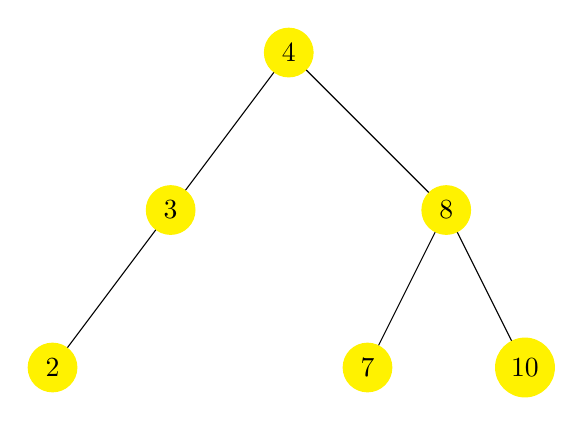
\begin{tikzpicture}[every node/.style={circle,draw=yellow, fill = yellow}]
    \node (4) {4};
      \node (3) at (-1.5, -2) {3};
        \draw (4) -- (3);
      
      \node (2) at (-3, -4) {2};
        \draw (2) -- (3);
    
      \node(8) at (2, -2) {8};
        \draw (8) -- (4);
    
      \node (7) at (1, -4) {7};
        \draw (7) -- (8);
      
      \node (10) at (3, -4) {10};
        \draw (10) -- (8);
    \end{tikzpicture}
    &
    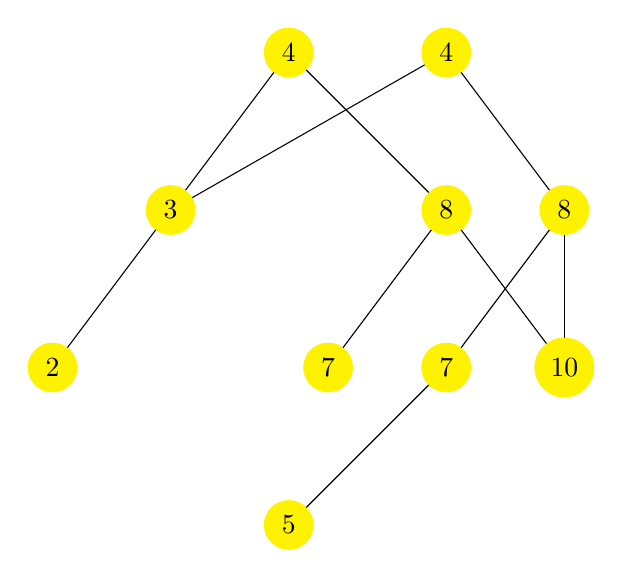
\begin{tikzpicture}[every node/.style={circle,draw=yellow,fill = yellow}]
      
      \node (A) {4};
      \node (B) at (-1.5, -2) {3};
        \draw (A) -- (B);
      
      \node (C) at (-3, -4) {2};
        \draw (C) -- (B);
    
      \node(D) at (2, -2) {8};
        \draw (A) -- (D);
    
      \node (E) at (0.5, -4) {7};
        \draw (D) -- (E);
      
      \node (F) at (3.5, -4) {10};
        \draw (D) -- (F);
      
      \node (A2) at (2, 0) {4};
        \draw (B) -- (A2);
    
      \node (D2) at (3.5, -2) {8};
        \draw (D2) -- (A2);
    
      \node (E2) at  (2, -4) {7};
        \draw (E2) -- (D2);
    
      \node (5) at (0, -6) {5};
        \draw (5) -- (E2);
    
        \draw (D2) -- (F);
        
    \end{tikzpicture}
    
    \end{tabular}\\\\
    
    \caption{\textbf{Figure 13.8 (a)} A binary search tree with keys 2, 3, 4, 7, 8, 10. \textbf{(b)} The persistent binary search tree that results from the insertion of key 5. The most recent version of the set consists of the nodes reachable from the root r', and the previous version consists of the nodes reachable from r. Blue nodes are added when key 5 is inserted.}
    
    \begin{description}
   
            \item[b.] Write a procedure PERSISTENT-TREE-INSERT(T,z) that, given a persistent binary search tree T and a node z to insert, returns a new persistent tree T' that is the result of inserting ´ into T. Assume that you have a procedure COPY-NODE(x) that makes a copy of node x, including all of its attributes.\\
            \item[c.]If the height of the persistent binary search tree T is h, what are the time and space requirements of your implementation of PERSISTENT-TREE-INSERT? (The space requirement is proportional to the number of nodes that are copied.)\\
            \item[d.] Suppose that you include the parent attribute in each node. In this case, the PERSISTENT-TREE-INSERT procedure needs to perform additional copying. Prove that PERSISTENT-TREE-INSERT then requires \SI{}{\ohm}(n) time and space, where n is the number of nodes in the tree.\\
            \item[e.]Show how to use red-black trees to guarantee that the worst-case running time and space are O(lg n) per insertion or deletion. You may assume that all keys are distinct.
        \end{description}

\end{document}
